\section{Brecha}

Los veinte papers del Anexo~\ref{anexo:papers}, leídos en cruz, dejan cinco cosas distintas. Casas et al.\ \cite{Casas2021} muestran el formato en 47 artículos, y Mainas et al.\ \cite{Mainas2023} prueban que el YAML se puede anotar. Shvaiko y Euzenat \cite{Shvaiko2005} dejan la taxonomía para cruzar esquemas. El Bayadh et al.\ \cite{ElBayadh2015} avisan que una medida no basta, y Santos Sousa et al.\ \cite{SantosSousa2026} dicen dónde fallan los embeddings: supervisión, escala, y pares que no son uno a uno. Schmidt y Thiry \cite{Schmidt2020} separan el dominio de la interfaz. BIAN puede ocupar ese lugar de referencia. Ehsan et al.\ \cite{Ehsan2022} y Golmohammadi et al.\ \cite{Golmohammadi2024} usan el contrato para probar APIs vivas. Mahanra Rao et al.\ \cite{MahanraRao2025} rankean servicios por calidad de servicio.

Casas y Mainas se quedan en el contrato. Shvaiko y El Bayadh no traen un YAML de banco. Schmidt separa el dominio de la interfaz y no calcula el desfase. Nosotros ponemos el Service Domain al lado del archivo y guardamos el AlignmentScore, para que otro pueda repetir el número.

\begin{table}[ht]
  \centering
  \caption{Vacíos V1 a V5}
  \label{tab:vacios}
  \footnotesize
  \begin{tabular}{@{}p{0.22\textwidth}p{0.34\textwidth}p{0.34\textwidth}@{}}
    \toprule
    Vacío & De dónde sale & Qué hacemos con eso \\
    \midrule
    V1. OpenAPI y BIAN juntos & El review no estudia los dos artefactos en banca & El objeto sigue siendo el contrato. BIAN es la referencia, y ese cruce no está en el review \\
    V2. Una métrica sola no alcanza & E2 y E3 aportan técnicas sueltas & S, E, C y el AlignmentScore \\
    V3. Cobertura & El matching ontológico habla de cobertura, no de business objects BIAN dentro del YAML & CoverageScore \\
    V4. Un procedimiento que se repita & Mainas et al.\ arman RDF. No dejan un score ni un nivel & El prototipo del capítulo III \\
    V5. Antes del despliegue & E5 y E6 miran runtime o ranking & El score es documental \\
    \bottomrule
  \end{tabular}
\end{table}

\begin{figure}[ht]
  \centering
  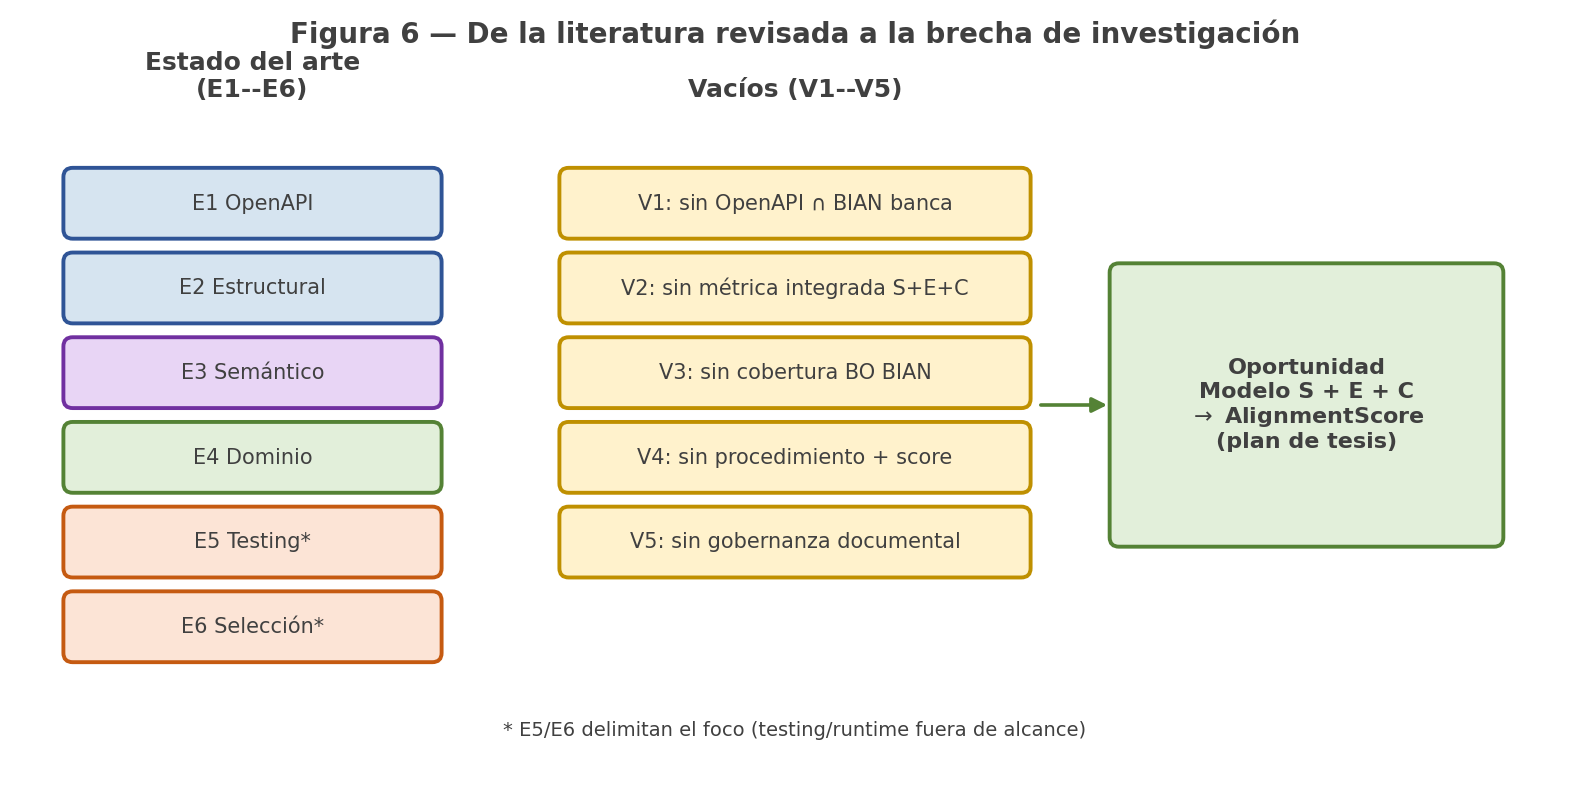
\includegraphics[width=0.92\textwidth]{Figura_06_Brecha}
  \caption{De los ejes E1--E6 a los vacíos V1--V5}
  \label{fig:brecha}
\end{figure}

\begin{figure}[ht]
  \centering
  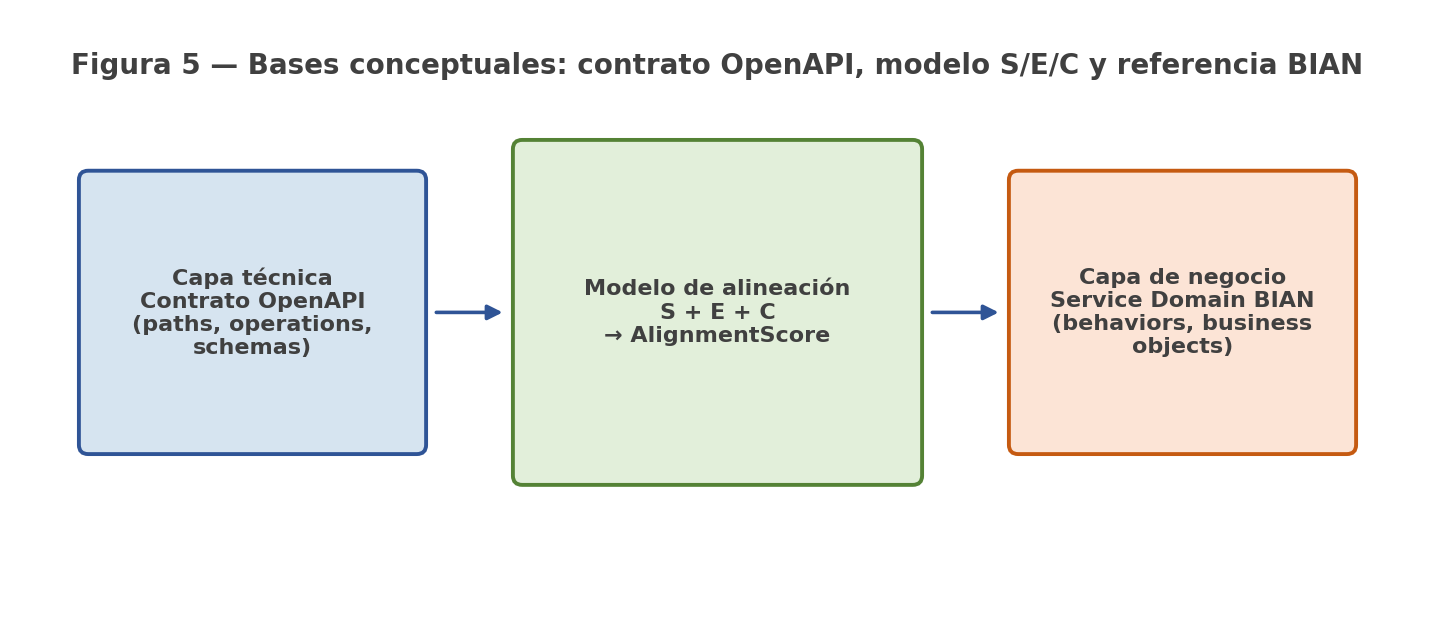
\includegraphics[width=0.88\textwidth]{Figura_05_Bases_Conceptuales}
  \caption{Contrato OpenAPI, Service Domain y modelo S/E/C}
  \label{fig:bases}
\end{figure}

He et al.\ \cite{He2022}, Schneider et al.\ \cite{Schneider2023} y Hertling y Paulheim \cite{Hertling2023} están en E3. Lu et al.\ \cite{Lu2024}, Kotstein y Decker \cite{Kotstein2024} y Oberle y Bauernhansl \cite{Oberle2024} están en E4. Entran como técnica del encoder y del parecido entre APIs. No arman el par contrato--Service Domain.
